%
% ---------------------------------------------------------------
% Copyright (C) 2012-2018 Gang Li
% ---------------------------------------------------------------
%
% This work is the default powerdot-tuliplab style test file and may be
% distributed and/or modified under the conditions of the LaTeX Project Public
% License, either version 1.3 of this license or (at your option) any later
% version. The latest version of this license is in
% http://www.latex-project.org/lppl.txt and version 1.3 or later is part of all
% distributions of LaTeX version 2003/12/01 or later.
%
% This work has the LPPL maintenance status "maintained".
%
% This Current Maintainer of this work is Gang Li.
%
%

\documentclass[
 size=14pt,
 paper=smartboard,  %a4paper, smartboard, screen
 mode=present, 		%present, handout, print
 display=slides, 	% slidesnotes, notes, slides
 style=tuliplab,  	% TULIP Lab style
 pauseslide,
 fleqn,leqno]{powerdot}

\usepackage{algorithm}
\usepackage{algorithmic}
\usepackage{cancel}
\usepackage{caption}
\usepackage{stackengine}
\usepackage{smartdiagram}
\usepackage{attrib}
\usepackage{amssymb}
\usepackage{amsmath} 
\usepackage{amsthm} 
\usepackage{mathtools}
\usepackage{rotating}
\usepackage{graphicx}
\usepackage{boxedminipage}
\usepackage{rotate}
\usepackage{calc}
\usepackage[absolute]{textpos}
\usepackage{psfrag,overpic}
\usepackage{fouriernc}
\usepackage{pstricks,pst-3d,pst-grad,pstricks-add,pst-text,pst-node,pst-tree}
\usepackage{moreverb,epsfig,subfigure}
\usepackage{color}
\usepackage{booktabs}
\usepackage{etex}
\usepackage{breqn}
\usepackage{multirow}
\usepackage{natbib}
\usepackage{bibentry}
\usepackage{gitinfo2}

%\usepackage{geometry}
%\geometry{verbose,letterpaper}
\usepackage{media9}
\usepackage{animate}
%\usepackage{movie15}
\usepackage{auto-pst-pdf}

\usepackage{breakurl}
\usepackage{fontawesome}
\usepackage{xcolor}
\usepackage{multicol}



\usepackage{verbatim}
\usepackage[utf8]{inputenc}
\usepackage{dtk-logos}
\usepackage{tikz}
\usepackage{adigraph}
%\usepackage{tkz-graph}
\usepackage{hyperref}
%\usepackage{ulem}
\usepackage{pgfplots}
\usepackage{verbatim}
\usepackage{fontawesome}
\usepackage{ragged2e}

\usepackage{todonotes}
% \usepackage{pst-rel-points}
\usepackage{animate}
\usepackage{fontawesome}

\usepackage{listings}
\lstset{frameround=fttt,
frame=trBL,
stringstyle=\ttfamily,
backgroundcolor=\color{yellow!20},
basicstyle=\footnotesize\ttfamily}
\lstnewenvironment{code}{
\lstset{frame=single,escapeinside=`',
backgroundcolor=\color{yellow!20},
basicstyle=\footnotesize\ttfamily}
}{}


\usepackage{hyperref}
\hypersetup{ % TODO: PDF meta Data
  pdftitle={Presentation Title},
  pdfauthor={Jingbao Luo},
  pdfpagemode={FullScreen},
  pdfborder={0 0 0}
}


% \usepackage{auto-pst-pdf}
% package to show source code

\definecolor{LightGray}{rgb}{0.9,0.9,0.9}
\newlength{\pixel}\setlength\pixel{0.000714285714\slidewidth}
\setlength{\TPHorizModule}{\slidewidth}
\setlength{\TPVertModule}{\slideheight}
\newcommand\highlight[1]{\fbox{#1}}
\newcommand\icite[1]{{\footnotesize [#1]}}

\newcommand\twotonebox[2]{\fcolorbox{pdcolor2}{pdcolor2}
{#1\vphantom{#2}}\fcolorbox{pdcolor2}{white}{#2\vphantom{#1}}}
\newcommand\twotoneboxo[2]{\fcolorbox{pdcolor2}{pdcolor2}
{#1}\fcolorbox{pdcolor2}{white}{#2}}
\newcommand\vpspace[1]{\vphantom{\vspace{#1}}}
\newcommand\hpspace[1]{\hphantom{\hspace{#1}}}
\newcommand\COMMENT[1]{}

\newcommand\placepos[3]{\hbox to\z@{\kern#1
        \raisebox{-#2}[\z@][\z@]{#3}\hss}\ignorespaces}

\renewcommand{\baselinestretch}{1.2}


\newcommand{\draftnote}[3]{
	\todo[author=#2,color=#1!30,size=\footnotesize]{\textsf{#3}}	}
% TODO: add yourself here:
%
\newcommand{\gangli}[1]{\draftnote{blue}{GLi:}{#1}}
\newcommand{\shaoni}[1]{\draftnote{green}{sn:}{#1}}
\newcommand{\gliMarker}
	{\todo[author=GLi,size=\tiny,inline,color=blue!40]
	{Gang Li has worked up to here.}}
\newcommand{\snMarker}
	{\todo[author=Sn,size=\tiny,inline,color=green!40]
	{Shaoni has worked up to here.}}

%%%%%%%%%%%%%%%%%%%%%%%%%%%%%%%%%%%%%%%%%%%%%%%%%%%%%%%%%%%%%%%%%%%%%%%%
% title
% TODO: Customize to your Own Title, Name, Address
%
\title{Flip01 Project}
\author{
Jingbao Luo
\\
\\Nanjing University of Science and Technology
}
\date{\gitCommitterDate}


% Customize the setting of slides
\pdsetup{
% TODO: Customize the left footer, and right footer
rf=\href{http://www.tulip.org.au}{
Last Changed by: \textsc{\gitCommitterName}\ \gitVtagn-\gitAbbrevHash\ (\gitAuthorDate)
},
cf={Flip01 Project},
}


\begin{document}

\maketitle

%\begin{slide}{Overview}
%\tableofcontents[content=sections]
%\end{slide}


%%==========================================================================================
%%
\begin{slide}[toc=,bm=]{Overview}
\tableofcontents[content=currentsection,type=1]
\end{slide}
%%
%%==========================================================================================


\section{Introduction}


%%==========================================================================================
%%
\begin{slide}{Introduction}

\begin{justify}
\setlength{\parindent}{2em}
The main implementation in this projecct is utilizing the Isolation Forest algorithm to achieve credit card fraud detection. By continuously fine-tuning the algorithm through parameter adjustments, the article aims to improve the algorithm's performance.
\end{justify}


\begin{justify}
\setlength{\parindent}{2em}
This project utilizes a dataset sourced from Kaggle to implement credit card fraud detection. The dataset contains transaction information of European cardholders during September 2013, conducted through credit cards. The dataset covers transactions that occurred within a span of two days, with a total of 284,807 transactions. Among these transactions, there were 492 cases of fraud, making the dataset highly imbalanced, where the positive class (fraudulent transactions) accounts for only 0.172% of all transactions.
\end{justify}
%%==========================================================================================

\end{slide}


\section{Method}


%%==========================================================================================
%%
\begin{slide}{\textit{iForest}}
\begin{justify}
\setlength{\parindent}{2em}
The Isolation Forest algorithm, proposed in 2008 by Liu Fei, Zhou Zhihua, and others, does not rely on distance or density metrics to describe the differences between samples and other samples. Instead, it directly characterizes the so-called isolation level. Therefore, this algorithm is simple, efficient, and widely used in the industry.
\end{justify}
\begin{justify}
\setlength{\parindent}{2em}
The logic of the Isolation Forest algorithm is intuitive. It uses binary trees to split the data, and both sample selection and feature selection are performed using randomization. If a certain sample is an outlier, it may require very few iterations to be isolated.
\end{justify}
\begin{figure}[H]
	\centering
	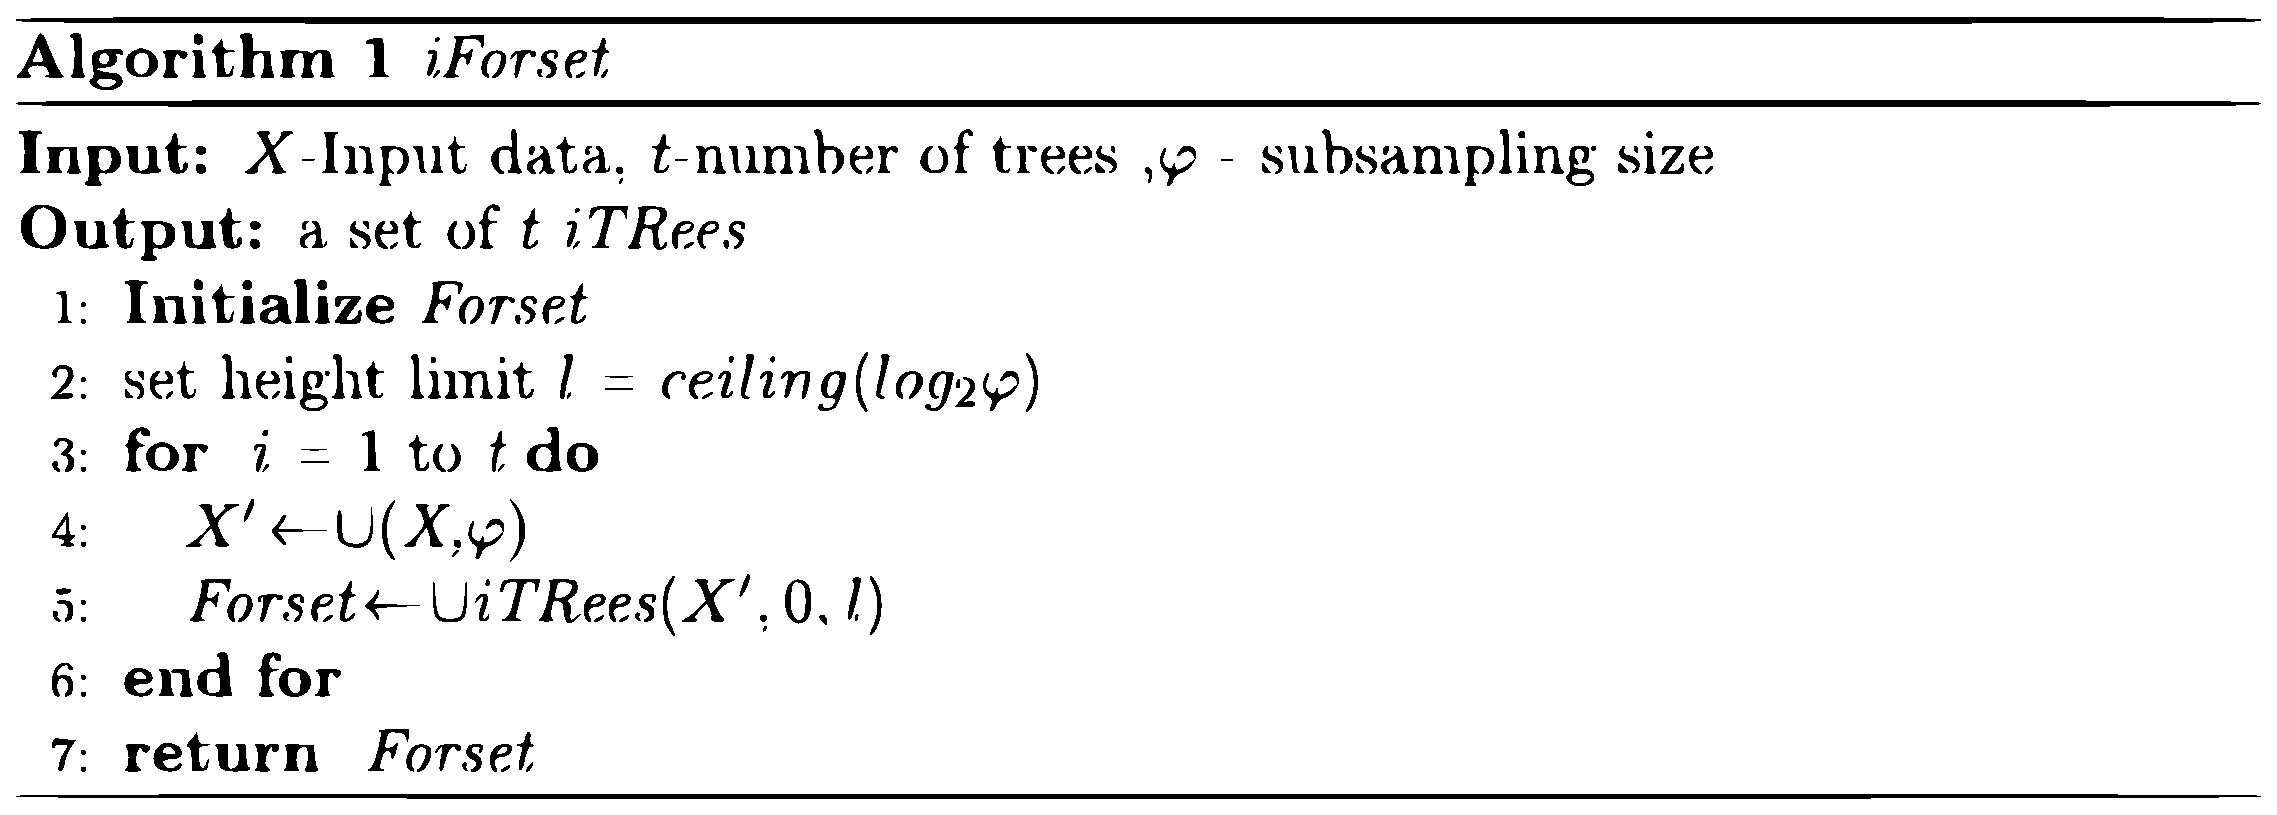
\includegraphics[width=0.7\textwidth]{figures/agm.eps}
	\label{fig:agm}
\end{figure}
\end{slide}
%%
%%==========================================================================================




\section{Data Exploration}


%%==========================================================================================
%%
\begin{slide}[toc=,bm=]{Data Description}
	
\begin{justify}
	\setlength{\parindent}{2em}	
	
Table provides a basic overview of the data for each attribute, including measures such as the mean, maximum, minimum, and other indicators.
\end{justify}





\begin{table}  \centering
	
	\caption{Data description}
	\label{tbl:data-description}
	\resizebox{\textwidth}{!}
	{
		\begin{tabular}{cccccccccccccccccccccccccccccccc}
			& Time        & V1          & V2          & V3          & V4          & V5          & V6          & V7          & V8          & V9          & V10         & V11         & V12         & V13         & V14         & V15         & V16         & V17         & V18         & V19         & V20         & V21         & V22         & V23         & V24         & V25         & V26         & V27         & V28         & Amount      & Class       \\
			count & 284807.0000 & 284807.0000 & 284807.0000 & 284807.0000 & 284807.0000 & 284807.0000 & 284807.0000 & 284807.0000 & 284807.0000 & 284807.0000 & 284807.0000 & 284807.0000 & 284807.0000 & 284807.0000 & 284807.0000 & 284807.0000 & 284807.0000 & 284807.0000 & 284807.0000 & 284807.0000 & 284807.0000 & 284807.0000 & 284807.0000 & 284807.0000 & 284807.0000 & 284807.0000 & 284807.0000 & 284807.0000 & 284807.0000 & 284807.0000 & 284807.0000 \\
			mean  & 94813.8596  & 0.0000      & 0.0000      & 0.0000      & 0.0000      & 0.0000      & 0.0000      & 0.0000      & 0.0000      & 0.0000      & 0.0000      & 0.0000      & 0.0000      & 0.0000      & 0.0000      & 0.0000      & 0.0000      & 0.0000      & 0.0000      & 0.0000      & 0.0000      & 0.0000      & 0.0000      & 0.0000      & 0.0000      & 0.0000      & 0.0000      & 0.0000      & 0.0000      & 88.3496     & 0.0017      \\
			std   & 47488.1460  & 1.9587      & 1.6513      & 1.5163      & 1.4159      & 1.3802      & 1.3323      & 1.2371      & 1.1944      & 1.0986      & 1.0888      & 1.0207      & 0.9992      & 0.9953      & 0.9586      & 0.9153      & 0.8763      & 0.8493      & 0.8382      & 0.8140      & 0.7709      & 0.7345      & 0.7257      & 0.6245      & 0.6056      & 0.5213      & 0.4822      & 0.4036      & 0.3301      & 250.1201    & 0.0415      \\
			min   & 0.0000      & -56.4075    & -72.7157    & -48.3256    & -5.6832     & -113.7433   & -26.1605    & -43.5572    & -73.2167    & -13.4341    & -24.5883    & -4.7975     & -18.6837    & -5.7919     & -19.2143    & -4.4989     & -14.1299    & -25.1628    & -9.4987     & -7.2135     & -54.4977    & -34.8304    & -10.9331    & -44.8077    & -2.8366     & -10.2954    & -2.6046     & -22.5657    & -15.4301    & 0.0000      & 0.0000      \\
			0.25  & 54201.5000  & -0.9204     & -0.5985     & -0.8904     & -0.8486     & -0.6916     & -0.7683     & -0.5541     & -0.2086     & -0.6431     & -0.5354     & -0.7625     & -0.4056     & -0.6485     & -0.4256     & -0.5829     & -0.4680     & -0.4837     & -0.4988     & -0.4563     & -0.2117     & -0.2284     & -0.5424     & -0.1618     & -0.3546     & -0.3171     & -0.3270     & -0.0708     & -0.0530     & 5.6000      & 0.0000      \\
			0.5   & 84692.0000  & 0.0181      & 0.0655      & 0.1798      & -0.0198     & -0.0543     & -0.2742     & 0.0401      & 0.0224      & -0.0514     & -0.0929     & -0.0328     & 0.1400      & -0.0136     & 0.0506      & 0.0481      & 0.0664      & -0.0657     & -0.0036     & 0.0037      & -0.0625     & -0.0295     & 0.0068      & -0.0112     & 0.0410      & 0.0166      & -0.0521     & 0.0013      & 0.0112      & 22.0000     & 0.0000      \\
			0.75  & 139320.5000 & 1.3156      & 0.8037      & 1.0272      & 0.7433      & 0.6119      & 0.3986      & 0.5704      & 0.3273      & 0.5971      & 0.4539      & 0.7396      & 0.6182      & 0.6625      & 0.4931      & 0.6488      & 0.5233      & 0.3997      & 0.5008      & 0.4589      & 0.1330      & 0.1864      & 0.5286      & 0.1476      & 0.4395      & 0.3507      & 0.2410      & 0.0910      & 0.0783      & 77.1650     & 0.0000      \\
			max   & 172792.0000 & 2.4549      & 22.0577     & 9.3826      & 16.8753     & 34.8017     & 73.3016     & 120.5895    & 20.0072     & 15.5950     & 23.7451     & 12.0189     & 7.8484      & 7.1269      & 10.5268     & 8.8777      & 17.3151     & 9.2535      & 5.0411      & 5.5920      & 39.4209     & 27.2028     & 10.5031     & 22.5284     & 4.5845      & 7.5196      & 3.5173      & 31.6122     & 33.8478     & 25691.1600  & 1.0000     
		\end{tabular}
	}
\end{table}

\end{slide}
%%
%%==========================================================================================


%%==========================================================================================
%%
\begin{slide}{Data Visualization}



\begin{figure}[H]
	\centering
	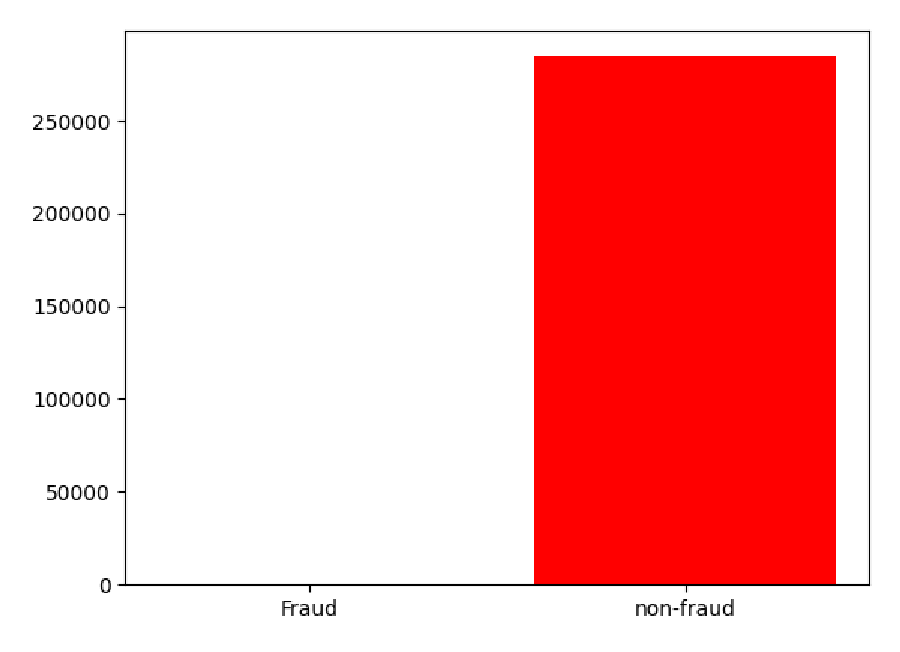
\includegraphics[width=0.7\textwidth]{figures/fraud.eps}
	\caption{fraud or no fraud}
	\label{fig:fraud data}
\end{figure}


\end{slide}
%%
%%==========================================================================================

\begin{slide}{Data Visualization}
	
	
	\begin{figure}[H]
		\centering
		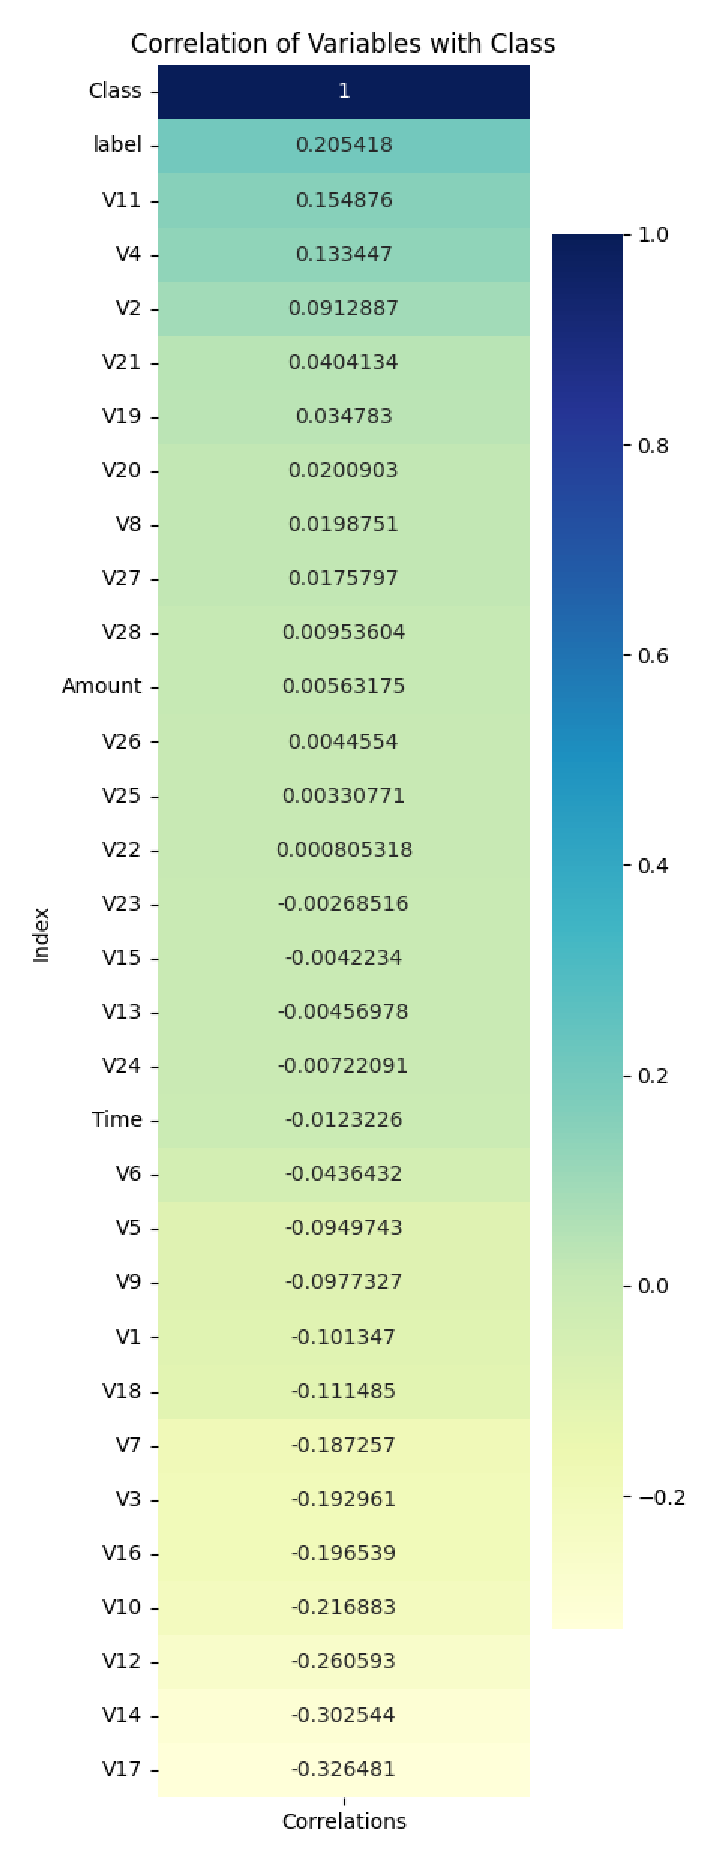
\includegraphics[height=0.6\textheight]{figures/correlation.eps}
		\caption{correlation heat plot}
		\label{fig:correlation}
	\end{figure}
	
\end{slide}
%%==========================================================================================
%%


\section{Experiment}


%%==========================================================================================
%%
\begin{slide}[toc=,bm=]{Experiment}

In the experimental design, we achieved the optimal performance of the model by continuously adjusting parameters. The evaluation of the training set's accuracy and recall mainly involved removing attributes and continuously changing the parameters of the isolation forest.

\begin{table}\centering
	
	\caption{parameter adjustment}
	\label{tbl:parameter-adjustment}
	\resizebox{\textwidth}{!}{
		\begin{tabular}{cccccc}
			\toprule
			Parameter & Accuarcy & Recall & Parameter & Accuarcy & Recall\\
			\midrule
			none-parameter-adjust & 0.963 & 0.821  & none-parameter-adjust(feature \_delete) & 0.953 & 0.663 \\
			n\_estimators-adjust(220) & 0.981 & 0.722  & n\_estimators-adjust(feature \_delete)(140) & 0.980 & 0.520 \\
			n\_features-adjust(11) & 0.981 & 0.750  & n\_features-adjust(feature \_delete)(11) & 0.981 & 0.522 \\
			max\_samples-adjust & 0.981 & 0.829  & nmax\_samples-adjust(feature \_delete) & 0.980 & 0.634\\
			\bottomrule
		\end{tabular}
	}
\end{table}

\end{slide}
%%
%%==========================================================================================


%%==========================================================================================
%%
\begin{slide}{Parameter adjustment}

\begin{figure}
	\centering
	\subfigure[n\_estimators-adjust]{
		\begin{minipage}[b]{0.4\textwidth}
			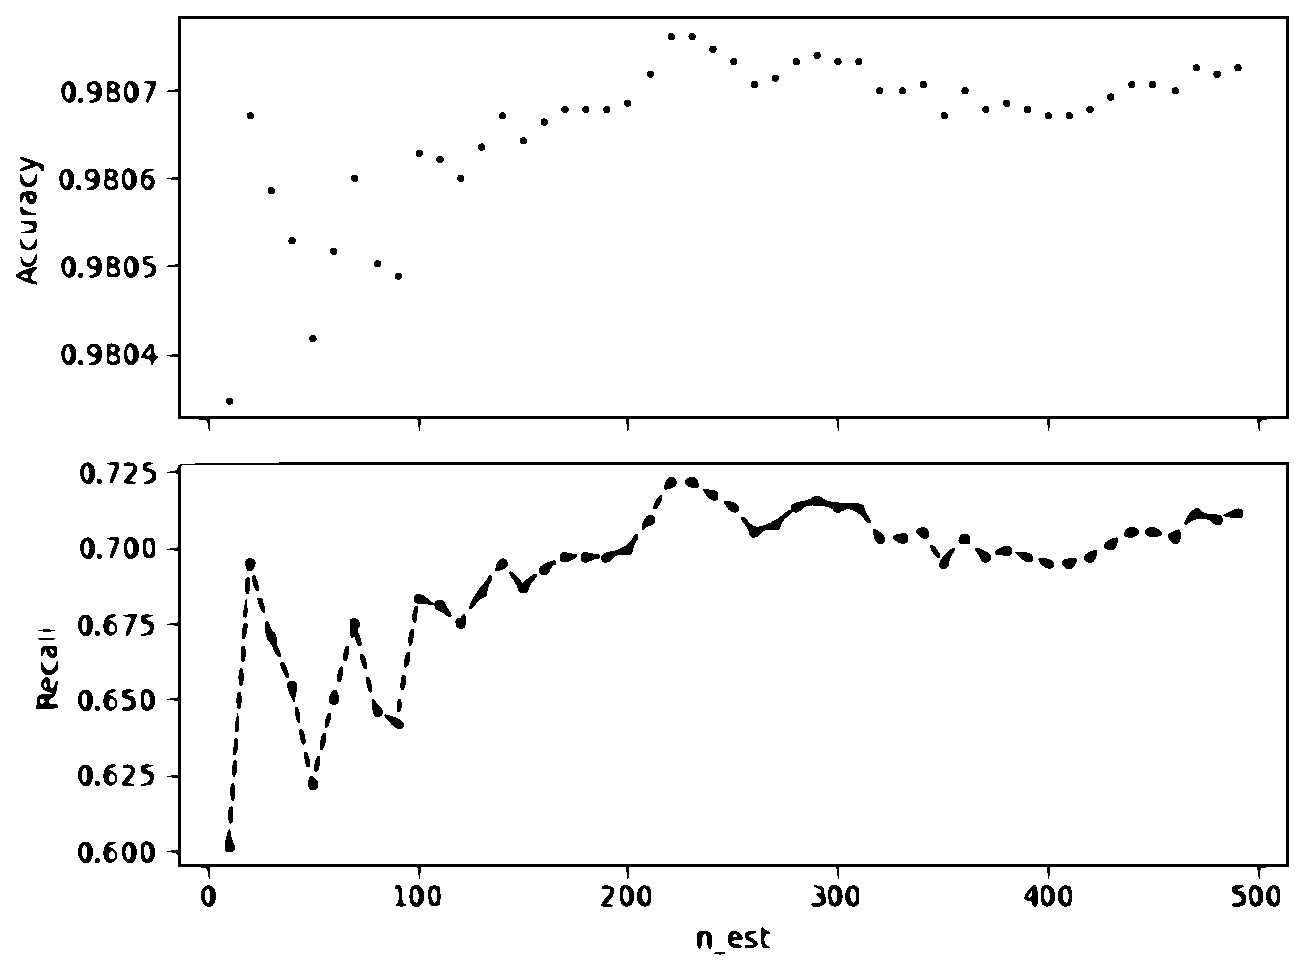
\includegraphics[width=1\textwidth]{figures/n_est_node.eps}
		\end{minipage}
		\label{fig:hor_2figs_1cap_2subcap_1}
	}
	\subfigure[n\_estimators-adjust (feature\_delete)]{
		\begin{minipage}[b]{0.4\textwidth}
			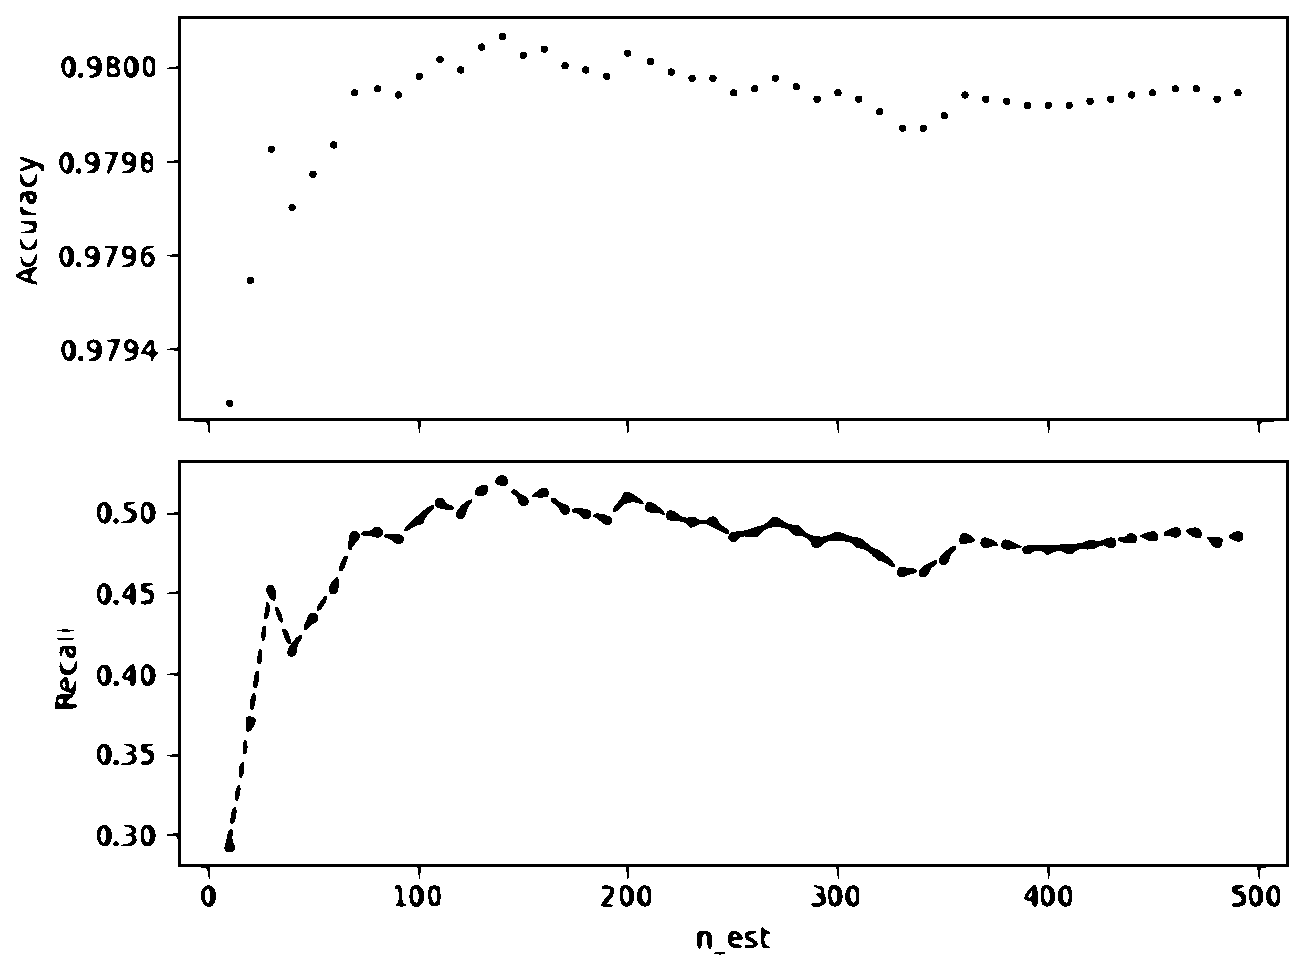
\includegraphics[width=1\textwidth]{figures/n_est.eps}
		\end{minipage}
		\label{fig:hor_2figs_1cap_2subcap_2}
	}
	\caption{n\_estimators-adjust}
	\label{fig:fig_n_estimators}
\end{figure}


\end{slide}
%%
%%==========================================================================================
\begin{slide}{Parameter adjustment}
	
	
	
	\begin{figure}
		\centering
		\subfigure[n\_features-adjust]{
			\begin{minipage}[b]{0.4\textwidth}
				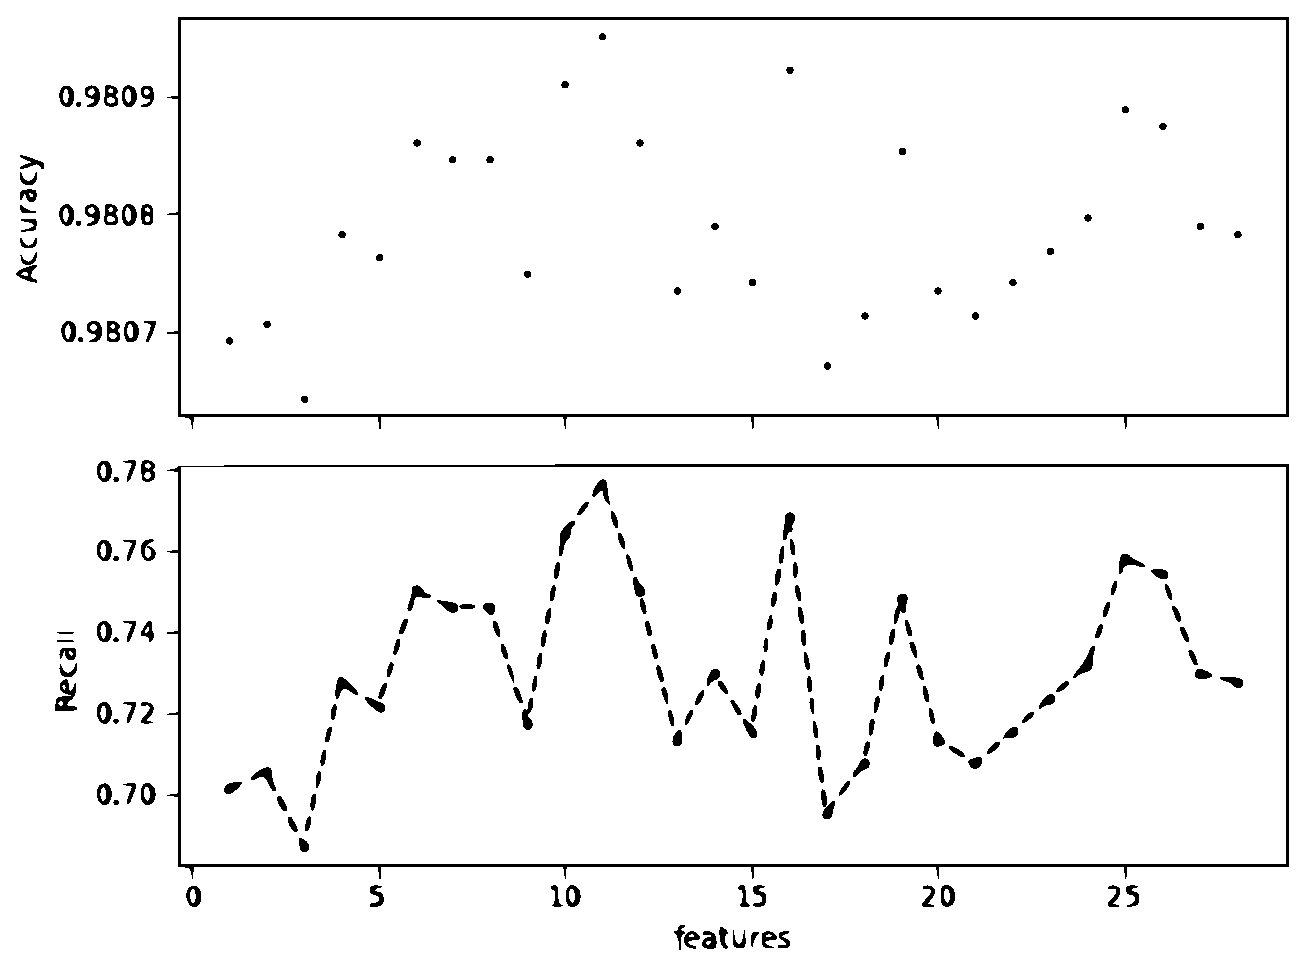
\includegraphics[width=1\textwidth]{figures/feature_nodelete.eps}
			\end{minipage}
			\label{fig:hor_2}
		}
		\subfigure[n\_features-adjust (feature\_delete)]{
			\begin{minipage}[b]{0.4\textwidth}
				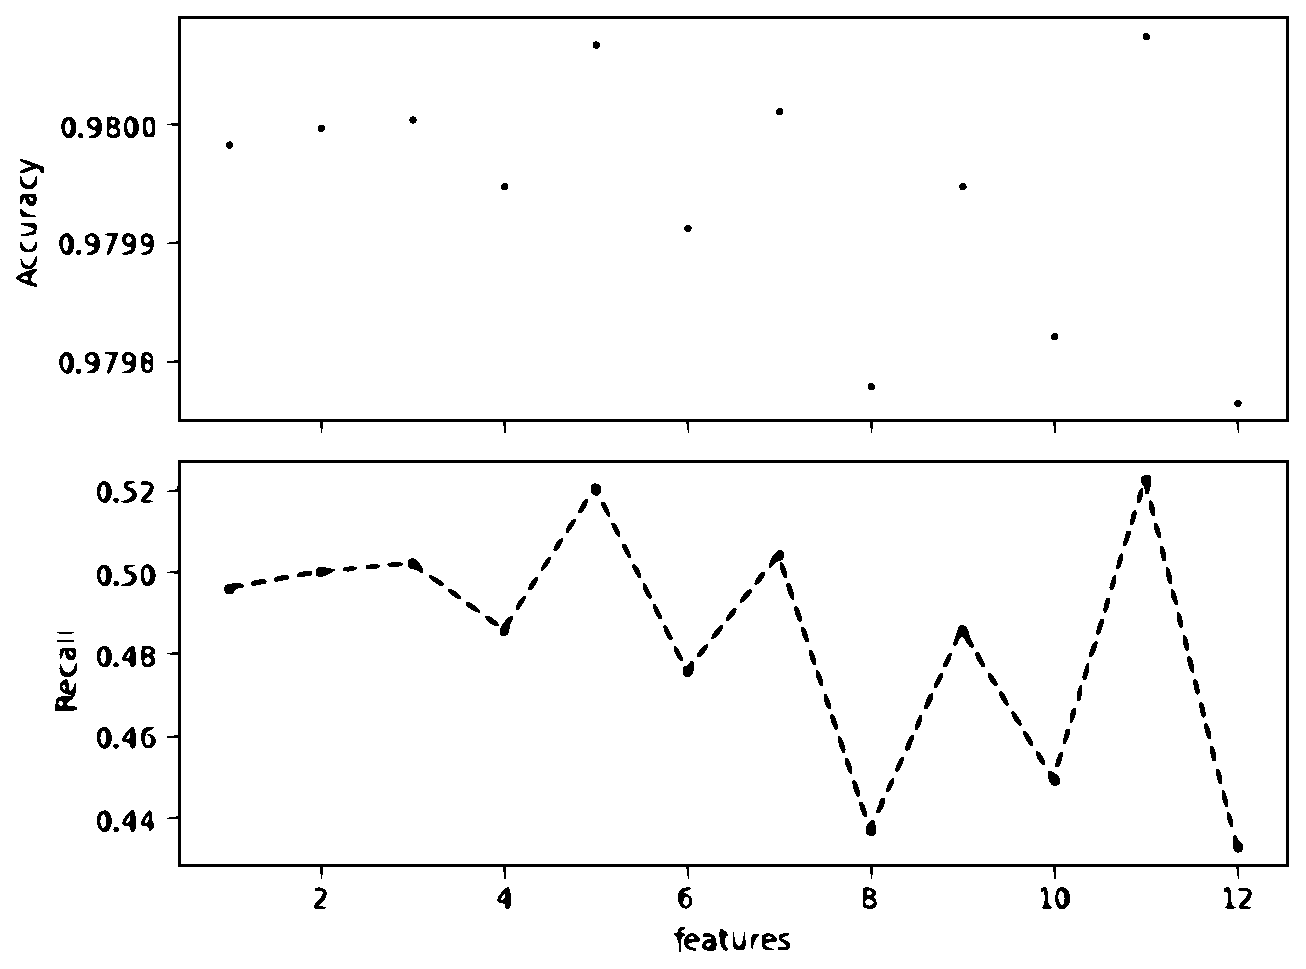
\includegraphics[width=1\textwidth]{figures/feature.eps}
			\end{minipage}
			\label{fig:hor}
		}
		\caption{n\_efeatures-adjust}
		\label{fig:n_features-adjust}
	\end{figure}
	
	
\end{slide}
%%
%%==========================================================================================
\begin{slide}{Parameter adjustment}
	
	
	
\begin{figure}
	\centering
	\subfigure[max\_samples-adjust]{
		\begin{minipage}[b]{0.4\textwidth}
			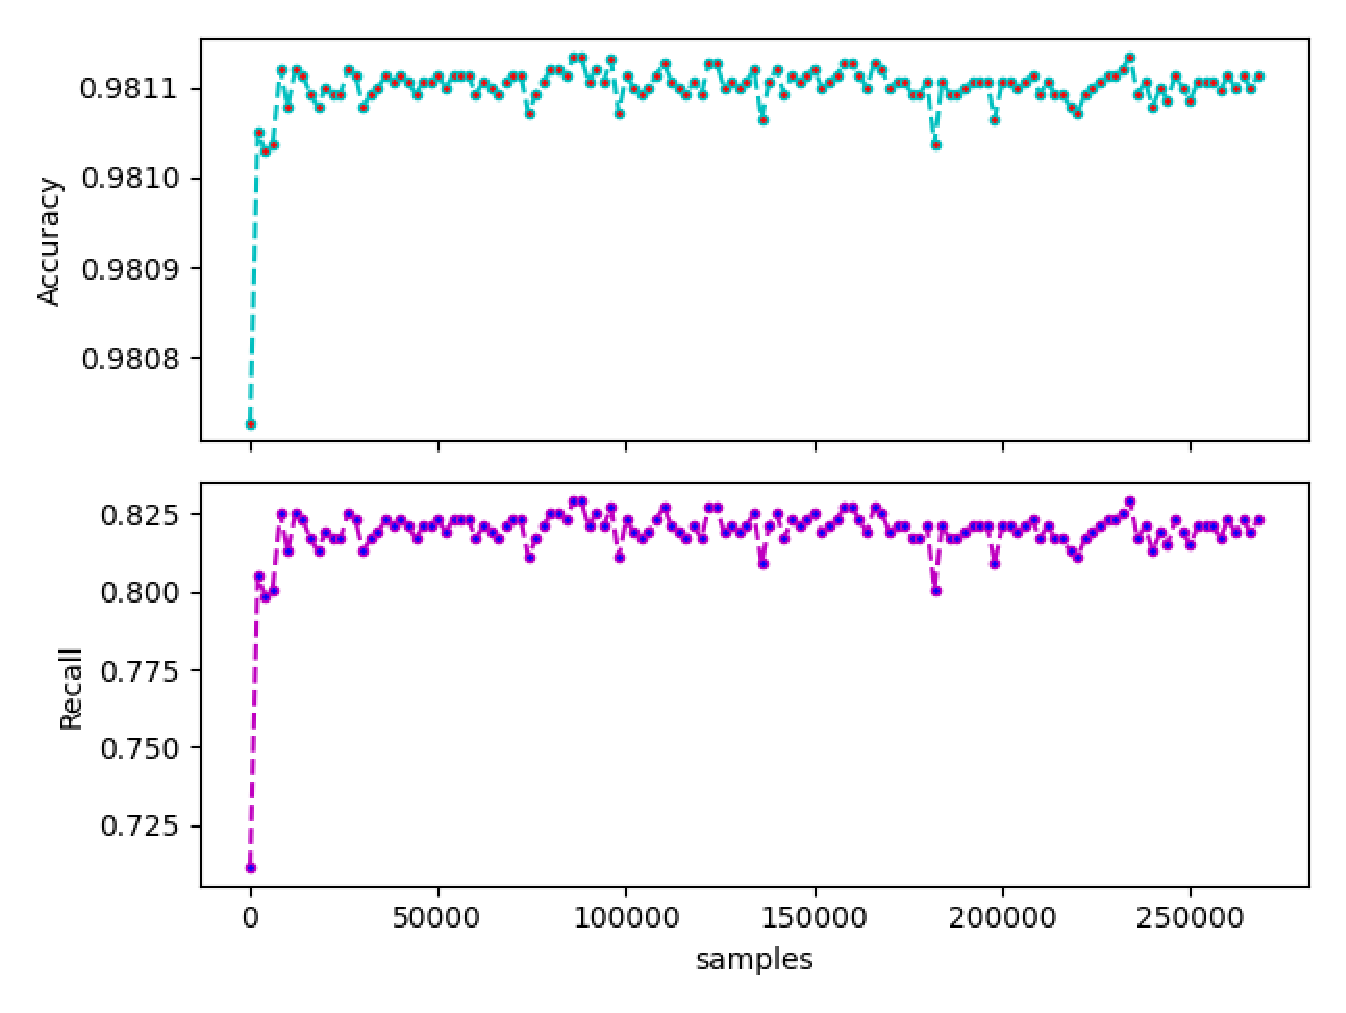
\includegraphics[width=1\textwidth]{figures/max_exampleN.eps}
		\end{minipage}
		\label{fig:h}
	}
	\subfigure[max\_samples-adjust (feature\_delete)]{
		\begin{minipage}[b]{0.4\textwidth}
			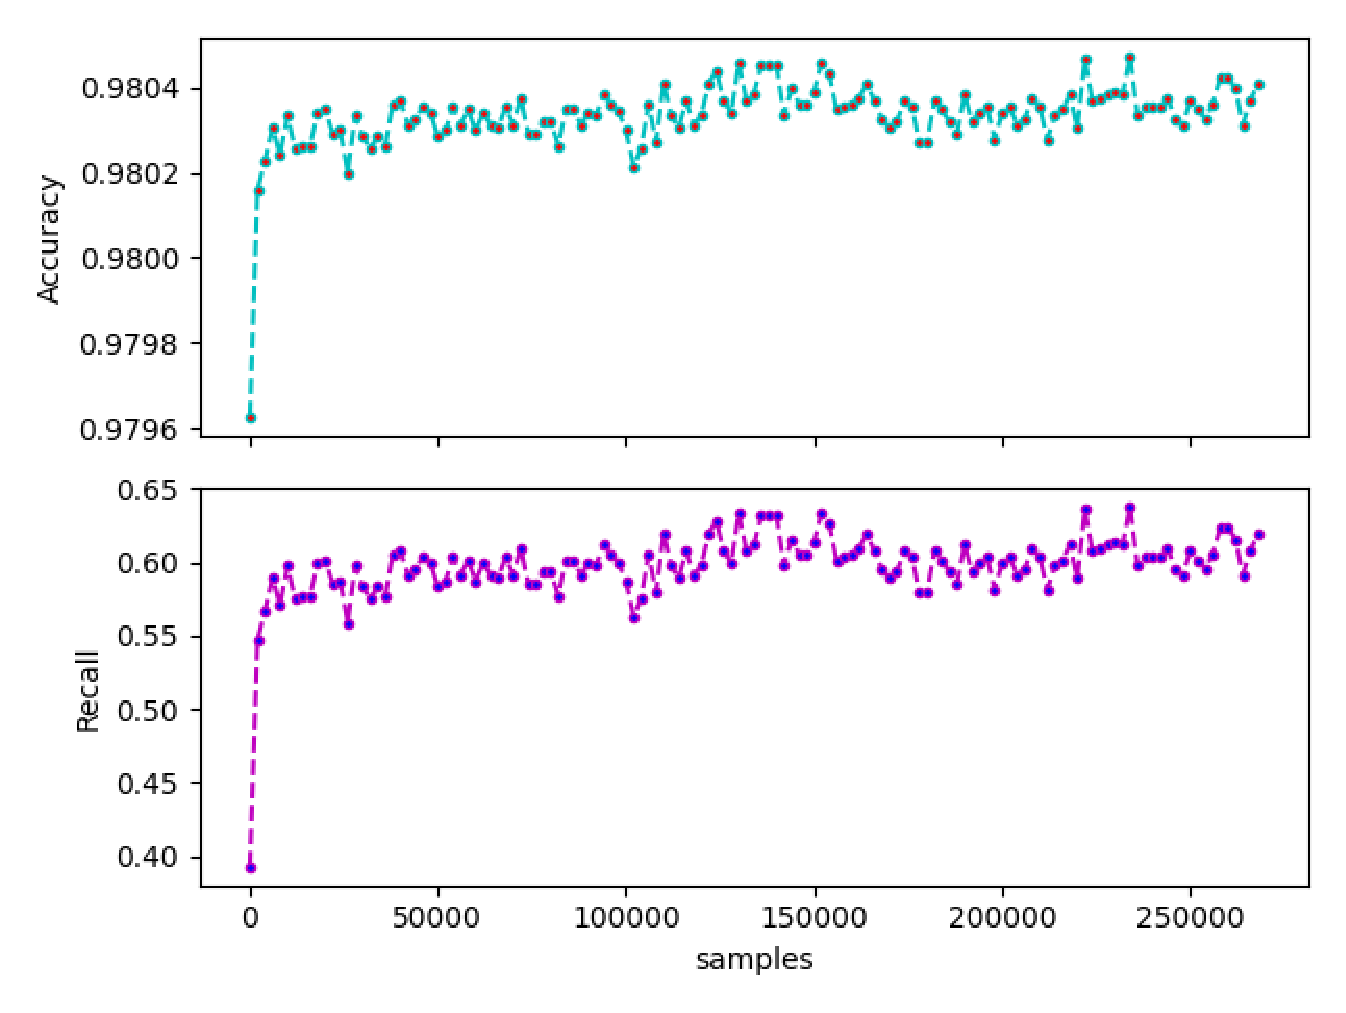
\includegraphics[width=1\textwidth]{figures/max_example.eps}
		\end{minipage}
		\label{fig:ho}
	}
	\caption{max\_samples-adjust}
	\label{fig:max_samples-adjust}
\end{figure}
	
	
\end{slide}
%%
%%==========================================================================================
\section{Conclusion}

%%==========================================================================================
%%
\begin{slide}[toc=,bm=]{Conclusion}

\begin{justify}
	\setlength{\parindent}{2em}
	The detection of credit card fraud data was achieved through Isolation Forest, and by continuously adjusting the parameters of the algorithm, a high level of accuracy and recall was ultimately reached, at 0.98 and 0.8, respectively.
\end{justify}

\begin{justify}
	\setlength{\parindent}{2em}
	However, a notable drawback of this method is the lack of a more in-depth analysis of attributes. This could mean that in the data preprocessing stage or feature selection process, there was insufficient exploration, understanding, and utilization of attribute information relevant to fraud. While optimizing the accuracy and recall of the model is undoubtedly important, equal attention should also be given to the importance and correlation of attributes, as well as their role in fraud detection.
\end{justify}
%%==========================================================================================

\end{slide}


\end{document}

\endinput
